En ocasiones nos podemos encontrar problemas o ejercicios los cuales se desarrollan sobre una cuadrícula y presentan una de las siguientes variantes:

\begin{itemize}
	
	\item La primera variante del problema es la cantidad de caminos desde la esquina superior izquierda hasta la esquina inferior derecha de una cuadrícula de $n \times n$, con la restricción de que solo podemos movernos hacia abajo y hacia la derecha y que existen un grupo de celdas dentro de la cuadriculas no pueden ser visitadas.
	
	\begin{figure}[h!]
		\centering
		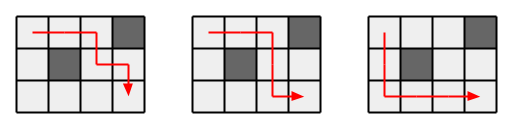
\includegraphics[width=0.7\linewidth]{img/grid_path_iii}
		\label{fig:gridpathiii}
	\end{figure}
	
	\item La segunda variante del problema es encontrar un camino desde la esquina superior izquierda hasta la esquina inferior derecha de una cuadrícula de $n \times n$, con la restricción de que solo podemos movernos hacia abajo y hacia la derecha. Cada cuadrado contiene un número entero y la ruta debe construirse de manera que la suma de los valores a lo largo de la ruta sea lo más grande posible.
	
	% TODO: \usepackage{graphicx} required
	\begin{figure}[h!]
		\centering
		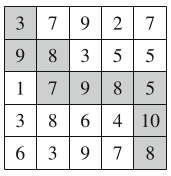
\includegraphics[width=0.3\linewidth]{img/grid_path_i}
		\label{fig:gridpathi}
	\end{figure}
	
	
	Como ejemplo, en la figura  muestra una ruta óptima en una cuadrícula de $5 \times 5$. La suma de los valores en la ruta es 67, y esta es la suma más grande posible en una ruta desde la esquina superior izquierda hasta la esquina inferior derecha.
	
\end{itemize}




De como resolver ambas variantes estará dedicada la siguiente guía de aprendizaje.